\documentclass[12pt]{article}
\usepackage{amsmath}
\usepackage{amsfonts}
\usepackage{enumerate}
\usepackage{pgfplots}
\usepackage{calc}
\usepackage{graphicx}
\usepackage{caption}
\usepackage{float}
\pgfplotsset{compat=1.12}
\begin{document}
\title{Computer Science M146, Homework 0}
\date{January 18th, 2018}
\author{Michael Wu\\UID: 404751542}
\maketitle

\section*{Problem 1}

\begin{align*}
        y&=x\sin(z)e^{-x}\\
        \frac{\partial y}{\partial x}&=\sin(z)e^{-x}-x\sin(z)e^{-x}\\
\end{align*}

\section*{Problem 2}

\[\mathbf{X}=\left(
        \begin{array}{@{}cc@{}}
                2&4\\
                1&3
        \end{array}
\right)\qquad
\mathbf{y}=\left(
        \begin{array}{@{}c@{}}
                1\\
                3
        \end{array}
\right)\qquad
\mathbf{z}=\left(
        \begin{array}{@{}c@{}}
                2\\
                3
        \end{array}
\right)
\]

\paragraph{a)}

\[\mathbf{y}^T\mathbf{z}=2\times 1+ 3\times 3 = 11\]

\paragraph{b)}

\[\mathbf{X}\mathbf{y}=\left(
        \begin{array}{@{}cc@{}}
                2&12\\
                1&9
        \end{array}
\right)\]

\paragraph{c)}

Yes it is invertible.

\[\mathbf{X}^{-1}=\frac{1}{2}\left(
        \begin{array}{@{}cc@{}}
                3&-4\\
                -1&2
        \end{array}
\right)\]

\paragraph{d)}

The rank is \(2\).

\section*{Problem 3}

\paragraph{a)}

The sample mean is \(\frac{3}{5}\).

\paragraph{b)}

\begin{align*}
        s^2&=\frac{1}{n-1}\sum_{i=1}{n}(x_i-\bar{x})^2\\
        &=\frac{1}{4}\left[2\left(\frac{3}{5}\right)^2+3\left(\frac{2}{5}\right)^2\right]\\
        &=\frac{3}{10}
\end{align*}

\paragraph{c)}

The probability is \(0.5^5=\frac{1}{32}\).

\paragraph{d)}

Let \(p=P\left(X_1=1\right)\). Then the probability of sample \(S\) occurring is
\[P(S)=p^3(1-p)^2\]
We can find maxima and minima using calculus.
\begin{align*}
        P^\prime(S)&=3p^2(1-p)^2-2p^3(1-p)\\
        P^\prime(S)&=3(p^2-2p^3+p^4)-2(p^3-p^4)\\
        P^\prime(S)&=5p^4-8p^3+3p^2\\
        P^\prime(S)&=p^2(5p^2-8p+3)\\
        P^\prime(S)&=p^2(5p-3)(p-1)\\
\end{align*}

The only critical point exists at \(p=\frac{3}{5}\), which must be the maxima. This is the value that
maximizes the probability of sample \(S\) occurring.

\paragraph{e)}

\[P(X=T|Y=b)=\frac{2}{5}\]

\section*{Problem 4}

\paragraph{a)}

False.

\paragraph{b)}

True.

\paragraph{c)}

False.

\paragraph{d)}

False.

\paragraph{e)}

True.

\section*{Problem 5}

\paragraph{a)} v
\paragraph{b)} iv
\paragraph{c)} ii
\paragraph{d)} i
\paragraph{e)} iii

\section*{Problem 6}

\paragraph{a)}

The mean is \(p\). The variance is \(p(1-p)\).

\paragraph{b)}

We begin with the definition of variance and note that the mean of \(X\) is \(0\), allowing us to write

\begin{align*}
        \operatorname{Var}(X)&=\operatorname{E}\left(X^2\right)-\operatorname{E}(X)^2\\
        &=\operatorname{E}\left(X^2\right)\\
        &=\sigma^2
\end{align*}

Because \(\operatorname{E}(X)=0\), we can find \(\operatorname{Var}(2X)\) similarly.

\begin{align*}
        \operatorname{Var}(2X)&=\operatorname{E}\left((2X)^2\right)-\operatorname{E}(2X)^2\\
        &=\operatorname{E}\left((2X)^2\right)\\
        &=4\operatorname{E}\left(X^2\right)\\
        &=4\sigma^2
\end{align*}

and similarly for \(\operatorname{Var}(X+2)\),

\begin{align*}
        \operatorname{Var}(X+2)&=\operatorname{E}\left((X+2)^2\right)-\operatorname{E}(X+2)^2\\
        &=\operatorname{E}\left(X^2+4X+4\right)-4\\
        &=\operatorname{E}\left(X^2\right)+\operatorname{E}(4X)+\operatorname{E}(4)-4\\
        &=\operatorname{E}\left(X^2\right)\\
        &=\sigma^2
\end{align*}

\section*{Problem 7}

\paragraph{a)}

\begin{enumerate}[i)]
        \item Both \(f(n)=O(g(n))\) and \(g(n)=O(f(n))\) are true. This is because
                \[f(n)=\ln(n)=\frac{\log_2(n)}{\log_2(e)}\]
                which is less than \(g(n)=\log_2(n)\) for all \(n>1\). In reverse, we have
                \[g(n)=\log_2(n)=\frac{\ln(n)}{\ln(2)}\]
                which is less than \(\frac{2}{\ln(2)}f(n)=2\frac{\ln(n)}{\ln(2)}\) for all \(n>1\).
        \item \(g(n)=O(f(n))\). \(f(n)\) is exponential while \(g(n)\) is polynomial.
        \item \(g(n)=O(f(n))\). \(f(n)>g(n)\) for all \(n>1\). \(f(n)\neq O(g(n))\) because for any positive constant \(c\),
                \[\frac{f(n)}{cg(n)}=c\left(\frac{3}{2}\right)^n\]
                which is an increasing function that will always surpass \(1\) as \(n\) becomes large. Thus \(f(n)\) will always
                outgrow any constant multiple of \(g(n)\).
\end{enumerate}

\paragraph{b)}

Use a binary search algorithm. Begin by checking the location halfway through the array, if it contains a zero with a one following it
we have the transition index. If it is a zero with a zero following it, move to the location halfway through the latter half of the array.
Otherwise if it is a one with a one following it, check the location halfway through the beginning half of the array. In this new location check
if it contains a zero with a one following it in order to determine if it is the transition index. Otherwise recursively continue checking and moving halfway
through the unchecked parts of the array, moving up or down depending on whether ones or zeros were found, until the transition index is found. This algorithm
is correct because each iteration removes half the array from being searched, and it only terminates upon finding the transition index. It never removes the transition
location, so eventually it will terminate and produce the correct output. The runtime is \(O(\log(n))\) because each iteration doubles the size of the array that can be searched.
After \(x\) iterations, we can search an array of size \(2^x\). Thus for an array of size \(n=2^x\), we only require \(\log_2(n)=x\) iterations. Thus our runtime is logarithmic.

\section*{Problem 8}

\paragraph{a)}

\begin{align*}
        \operatorname{E}(XY)&=\sum_{x,y\in\mathbb{R}} xy\operatorname{P}(X=x)\operatorname{P}(Y=y)\\
        &=\sum_{x\in\mathbb{R}}x\operatorname{P}(X=x)\sum_{y\in\mathbb{R}}\operatorname{P}(Y=y)\\
        &=\operatorname{E}(X)\operatorname{E}(Y)
\end{align*}

\paragraph{b)}

\begin{enumerate}[i)]
        \item \(\operatorname{E}(\text{Number of }3\text{'s})=6000*\frac{1}{6}=1000\). The law of large numbers states that the
                results obtained from a large number of trials should be close to the expected value.
        \item The coin toss \(X\) has a Bernoulli distribution with \(p=\frac{1}{2}\), so its mean is \(\mu=p=\frac{1}{2}\) and its 
                variance is \(\sigma^2=p(1-p)=\frac{1}{4}\). The central limit theorem states that as \(n\) increases,
                \(\sqrt{n}\left(\bar{X}-\mu\right)\rightarrow\mathcal{N}\left(0,\sigma^2\right)\), thus
                \[\sqrt{n}\left(\bar{X}-\frac{1}{2}\right)\overset{n\to\infty}{\longrightarrow}\mathcal{N}\left(0,\frac{1}{4}\right)\]
\end{enumerate}

\section*{Problem 9}

\paragraph{a)}

\begin{enumerate}[i)]
        \item \(\left\lVert x\right\rVert_2\leq 1\)
        \begin{center}
                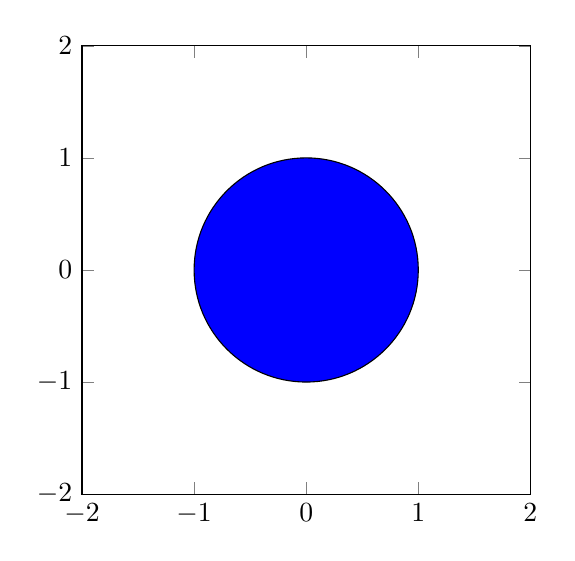
\begin{tikzpicture}
                        \begin{axis}[xmin=-2,xmax=2,ymin=-2,ymax=2,axis equal image]
                                \filldraw[fill=blue, draw=black] (axis cs:0,0) circle (1);
                        \end{axis}
                \end{tikzpicture}
        \end{center}

        \item \(\left\lVert x\right\rVert_0\leq 1\)
        \begin{center}
                \begin{tikzpicture}
                        \begin{axis}[xmin=-2,xmax=2,ymin=-2,ymax=2,axis equal image]
                                \draw[<->] (axis cs:2,0) -- (axis cs:-2,0);
                                \draw[<->] (axis cs:0,2) -- (axis cs:0,-2);
                        \end{axis}
                \end{tikzpicture}
        \end{center}

        \item \(\left\lVert x\right\rVert_1\leq 1\)
        \begin{center}
                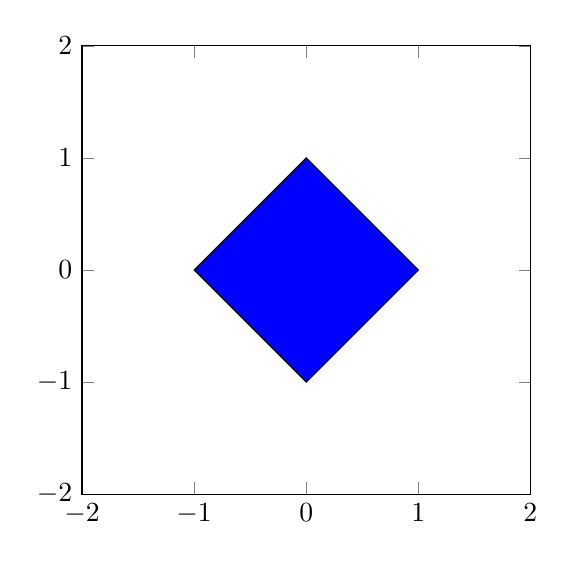
\begin{tikzpicture}
                        \begin{axis}[xmin=-2,xmax=2,ymin=-2,ymax=2,axis equal image]
                                \filldraw[fill=blue, draw=black] (axis cs:1,0) -- (axis cs:0,1) -- (axis cs:-1,0) -- (axis cs:0,-1) -- cycle;
                        \end{axis}
                \end{tikzpicture}
        \end{center}

        \item \(\left\lVert x\right\rVert_\infty\leq 1\)
        \begin{center}
                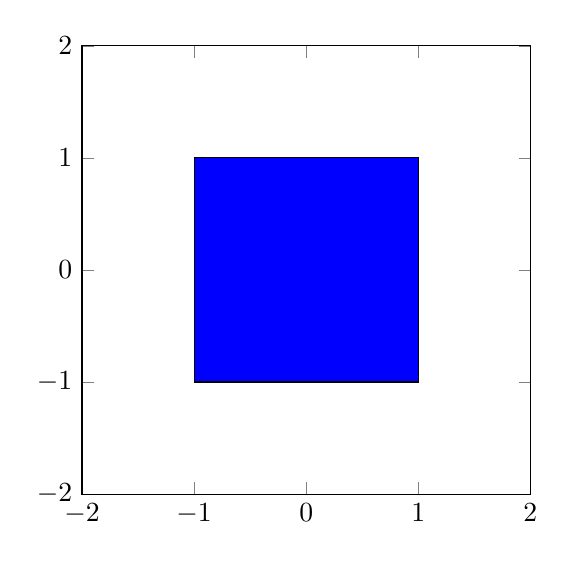
\begin{tikzpicture}
                        \begin{axis}[xmin=-2,xmax=2,ymin=-2,ymax=2,axis equal image]
                                \filldraw[fill=blue, draw=black] (axis cs:-1,-1) rectangle (axis cs:1,1);
                        \end{axis}
                \end{tikzpicture}
        \end{center}
\end{enumerate}

\paragraph{b)}

\begin{enumerate}[i)]
        \item Given a square matrix \(\mathbf{A}\), an eigenvector \(\vec{\mathbf{x}}\) is a vector such that
                \[\mathbf{A}\vec{\mathbf{x}}=\lambda\vec{\mathbf{x}}\]
                where \(\lambda\) is a scalar constant. \(\lambda\) is an eigenvalue of the matrix \(\mathbf{A}\).
        \item The characteristic equation is
                \[(2-\lambda)^2-1=\lambda^2-4\lambda+3=(\lambda-3)(\lambda-1)\]
                giving us eigenvalues \(\lambda_1=1\) and \(\lambda_2=3\). To find the eigenvectors we need to find the null space of
                \[\mathbf{A}_{\lambda_1}=\left(
                        \begin{array}{@{}cc@{}}
                                1&1\\
                                1&1
                        \end{array}
                \right)
                \qquad
                \mathbf{A}_{\lambda_2}=\left(
                        \begin{array}{@{}cc@{}}
                                -1&1\\
                                1&-1
                        \end{array}
                \right)\]
                This gives us eigenvectors \(\vec{\mathbf{x}}_1=\left<1,-1\right>\) and \(\vec{\mathbf{x}}_2=\left<1,1\right>\)
        \item Take any eigenvalue \(\lambda\) and eigenvector \(\vec{\mathbf{x}}\) pair of the matrix \(\mathbf{A}\). Then
                \begin{align*}
                        \mathbf{A}\vec{\mathbf{x}}&=\lambda\vec{\mathbf{x}}\\
                        \mathbf{A}^2\vec{\mathbf{x}}&=\lambda\mathbf{A}\vec{\mathbf{x}}=\lambda^2\vec{\mathbf{x}}\\
                        &\mathrel{\makebox[\widthof{=}]{\vdots}}\\
                        \mathbf{A}^k\vec{\mathbf{x}}&=\lambda^{k-1}\mathbf{A}\vec{\mathbf{x}}=\lambda^k\vec{\mathbf{x}}
                \end{align*}
                Thus \(\lambda^k\) and \(\vec{\mathbf{x}}\) form and eigenvalue and eigenvector pair for the matrix \(\mathbf{A}^k\). This
                holds for every eigenvalue and eigenvector pair, showing that the eigenvalues of \(\mathbf{A}^k\) are \(\lambda_1^k,\lambda_2^k,\ldots,\lambda_n^k\)
                and that each eigenvector of \(\mathbf{A}\) is still an eigenvector of \(\mathbf{A}^k\).
\end{enumerate}

\paragraph{c)}

\begin{enumerate}[i)]
        \item
                \[\frac{\partial\mathbf{a}^T\mathbf{x}}{\partial\mathbf{x}}=\mathbf{a}^T\]
        \item We find the first derivative by doing
                \begin{align*}
                        \frac{\partial\mathbf{x}^T\mathbf{Ax}}{\partial\mathbf{x}}&=\frac{\partial}{\partial\mathbf{x}}
                                \left(\begin{matrix}
                                        x_1 & x_2 & \ldots & x_n
                                \end{matrix}\right)
                                \left(\begin{matrix}
                                        a_{11} & a_{12} & \cdots & a_{1n}\\
                                        a_{21} & a_{22} &        &\\
                                        \vdots &        & \ddots &\\
                                        a_{n1} &        &        & a_{nn}
                                \end{matrix}\right)
                                \left(\begin{matrix}
                                        x_1\\
                                        x_2\\
                                        \vdots\\
                                        x_n
                                \end{matrix}\right)\\
                        &=\frac{\partial}{\partial\mathbf{x}}
                                \left(\begin{matrix}
                                        x_1 & x_2 & \ldots & x_n
                                \end{matrix}\right)
                                \left(\begin{matrix}
                                        a_{11}x_1+a_{12}x_2+\ldots+a_{1n}x_n\\
                                        a_{21}x_1+a_{22}x_2+\ldots+a_{2n}x_n\\
                                        \vdots\\
                                        a_{n1}x_1+a_{n2}x_2+\ldots+a_{nn}x_n
                                \end{matrix}\right)\\
                        &=\frac{\partial}{\partial\mathbf{x}}\left[\sum_{i=1}^{n} a_{ii}{x_i}^2 + \sum_{i,j\in (1,n), i\neq j} a_{ij} x_i x_j\right]\\
                        &=\left(\begin{matrix}
                                2a_{11}x_1 + 2a_{12}x_2 + \ldots + 2a_{1n}x_n\\
                                \vdots\\
                                2a_{n1}x_1 + 2a_{n2}x_2 + \ldots + 2a_{nn}x_n\\
                          \end{matrix}\right)^T\\
                        &=2
                                \left(\begin{matrix}
                                        x_1 & x_2 & \ldots & x_n
                                \end{matrix}\right)
                                \left(\begin{matrix}
                                        a_{11} & a_{12} & \cdots & a_{1n}\\
                                        a_{21} & a_{22} &        &\\
                                        \vdots &        & \ddots &\\
                                        a_{n1} &        &        & a_{nn}
                                \end{matrix}\right)\\
                        &=2\mathbf{x}^T\mathbf{A}
                \end{align*}
                We find the second derivative by doing
                \begin{align*}
                        \frac{\partial\mathbf{x}^T\mathbf{Ax}}{\partial\mathbf{x}^2}&=\frac{\partial}{\partial\mathbf{x}}2\mathbf{x}^T\mathbf{A}\\
                        &=2\mathbf{A}
                \end{align*}
\end{enumerate}

\paragraph{d)}

\begin{enumerate}[i)]
        \item Because \(\mathbf{w}^T\mathbf{x}+b=0\) is a line, both \(\mathbf{w}\) and \(\mathbf{x}\) must be vectors in \(\mathbb{R}^2\). Let \(\mathbf{x}_1\) and
                \(\mathbf{x}_2\) be points on the line. Then
                \begin{align*}
                        \mathbf{w}^T\mathbf{x}_1+b&=0\\
                        \mathbf{w}^T\mathbf{x}_2+b&=0\\
                        \mathbf{w}^T\left(\mathbf{x}_1-\mathbf{x}_2\right)&=0
                \end{align*}
                Thus \(\mathbf{w}\) is orthogonal to the line defined by \(\mathbf{w}^T\mathbf{x}+b=0\), because it is orthogonal to the vector \(\mathbf{x}_1-\mathbf{x}_2\) that
                lies along the line.
        \item The shortest distance to the line from the origin must be along a vector perpendicular to the line. Thus let
                \(\mathbf{x}=c\frac{\mathbf{w}}{\left\lVert \mathbf{w}\right\rVert_2}\). We need to solve
                \[c\frac{\mathbf{w}^T\mathbf{w}}{\left\lVert w\right\rVert_2}+b=0\]
                for \(c\) to find the distance to the origin. Because
                \(\mathbf{w}^T\mathbf{w}=\left\lVert \mathbf{w}\right\rVert_2^2\), we get \(c=-\frac{b}{\left\lVert \mathbf{w}\right\rVert_2}\).
                Taking the absolute value of this, we get the distance \(\frac{b}{\left\lVert \mathbf{w}\right\rVert_2}\) to the origin.
\end{enumerate}

\section*{Problem 10}

\paragraph{a)} See figure \(1\).

\begin{figure}[H]
        \begin{center}
                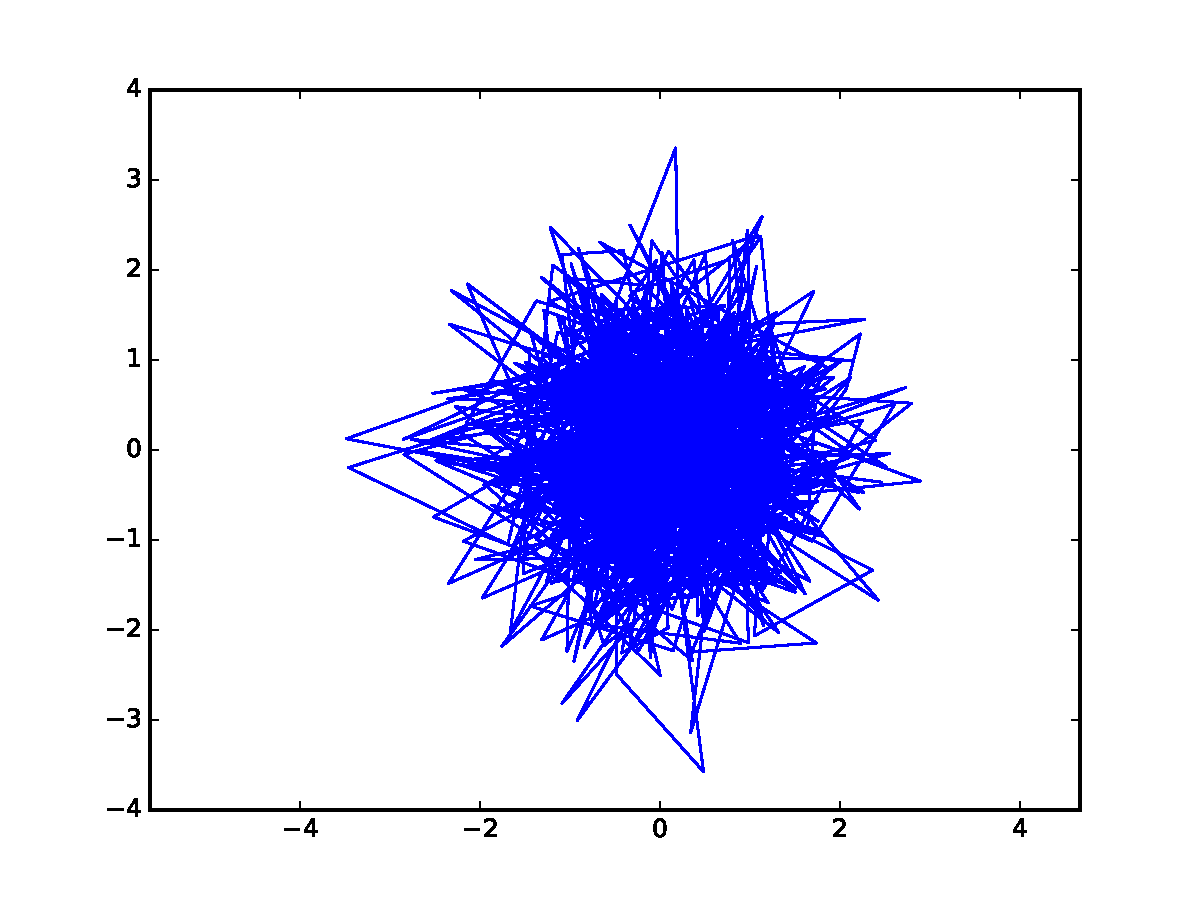
\includegraphics[height=2.5in]{Problem10-a}
                \caption{\(1000\) samples with mean \((0,0)\) and identity covariance matrix.}
        \end{center}
\end{figure}

\pagebreak

\paragraph{b)} See figure \(2\). The center shifts to \((1,1)\).

\begin{figure}[H]
        \begin{center}
                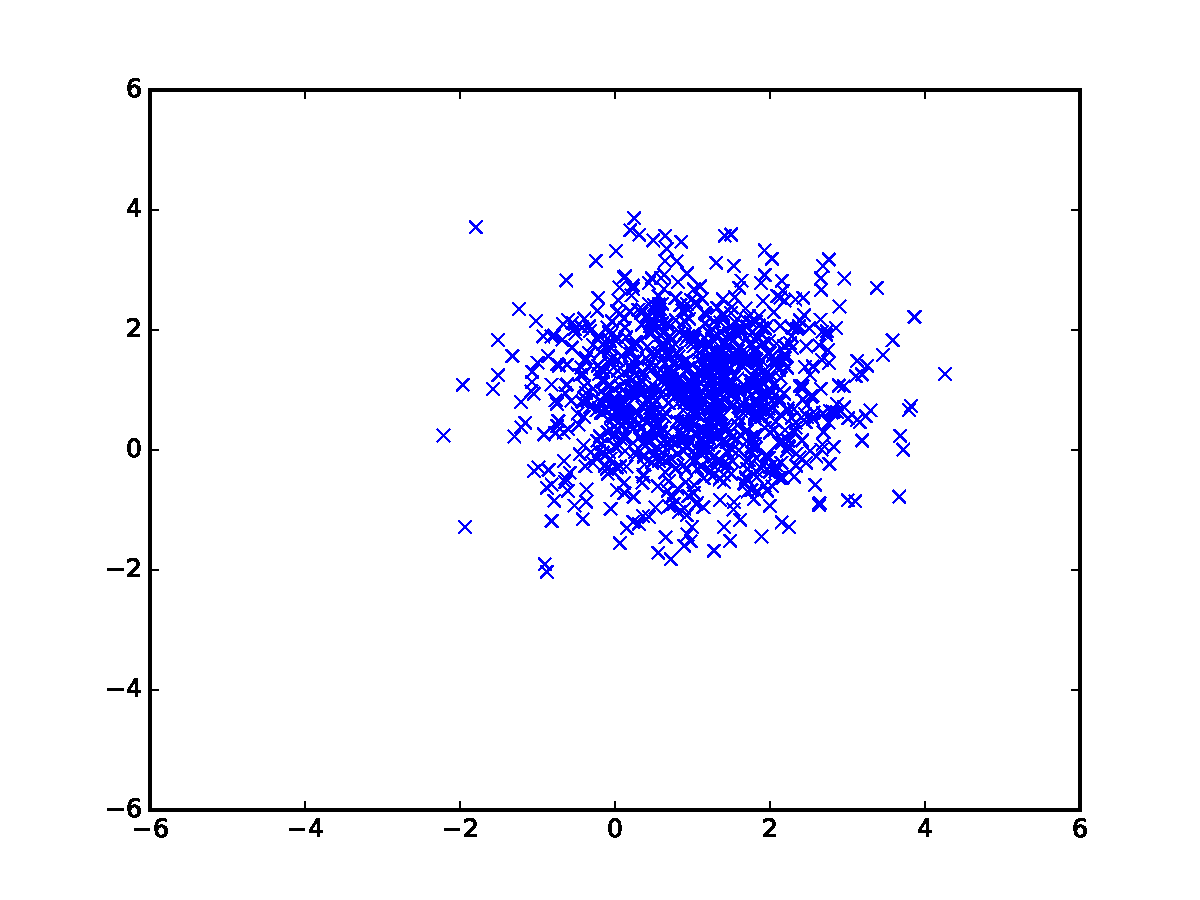
\includegraphics[height=2.5in]{Problem10-b}
                \caption{\(1000\) samples with mean \((1,1)\) and identity covariance matrix.}
        \end{center}
\end{figure}

\paragraph{c)} See figure \(3\). It becomes more spread out.

\begin{figure}[h!]
        \begin{center}
                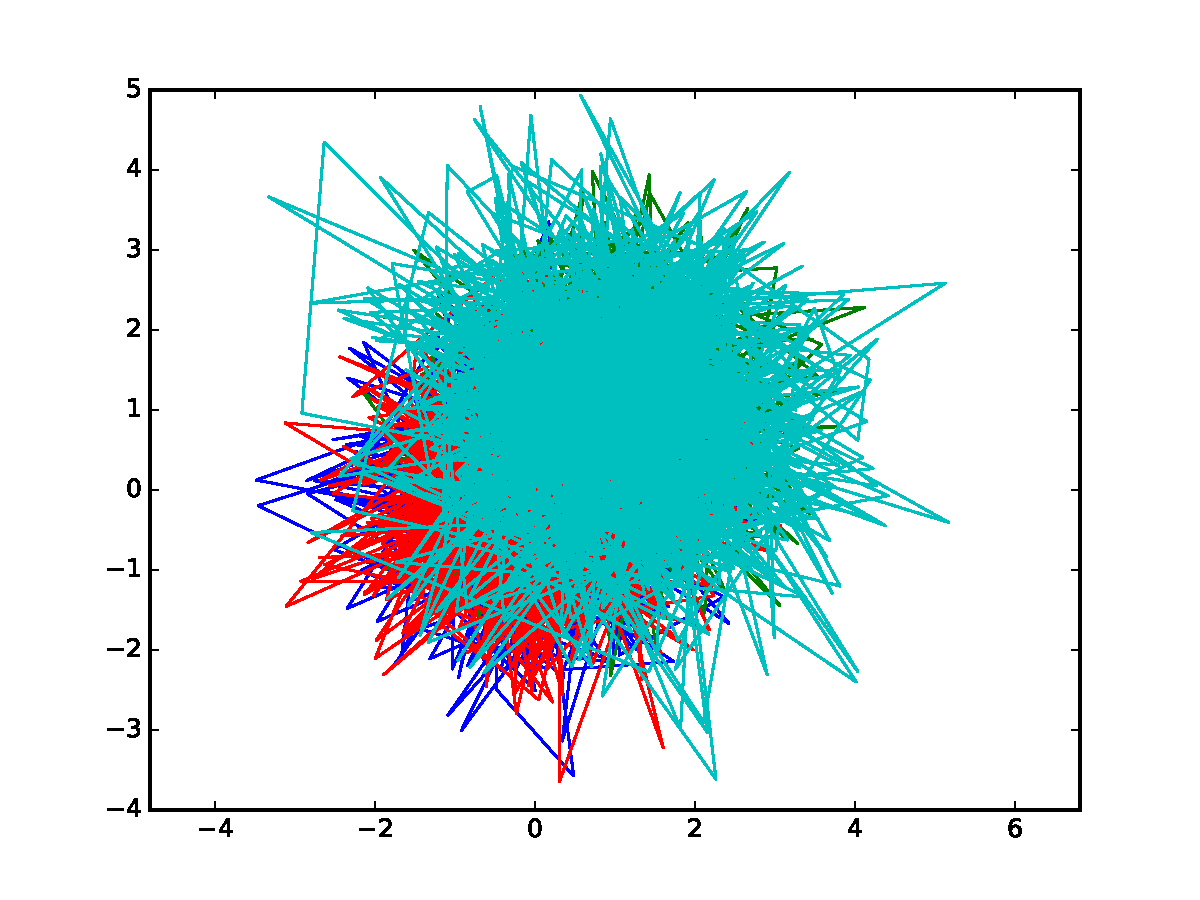
\includegraphics[height=2.5in]{Problem10-c}
                \caption{\(1000\) samples with mean \((0,0)\) and covariance matrix \(2I_2\).}
        \end{center}
\end{figure}

\paragraph{d)} See figure \(4\). \(x\) and \(y\) become positively correlated.

\begin{figure}[H]
        \begin{center}
                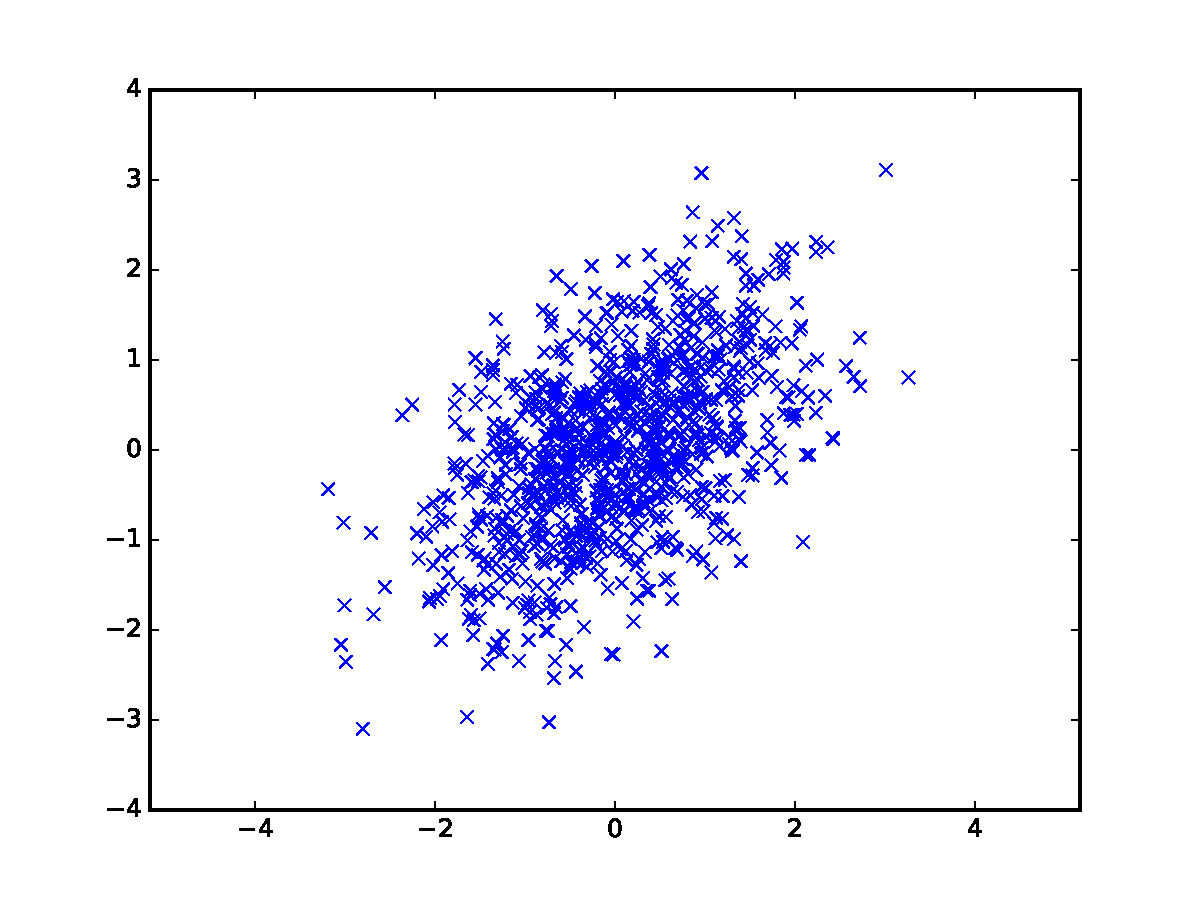
\includegraphics[height=2.5in]{Problem10-d}
                \caption{\(1000\) samples with mean \((0,0)\) and positively correlated covariance matrix.}
        \end{center}
\end{figure}

\paragraph{e)} See figure \(5\). \(x\) and \(y\) become negatively correlated.

\begin{figure}[H]
        \begin{center}
                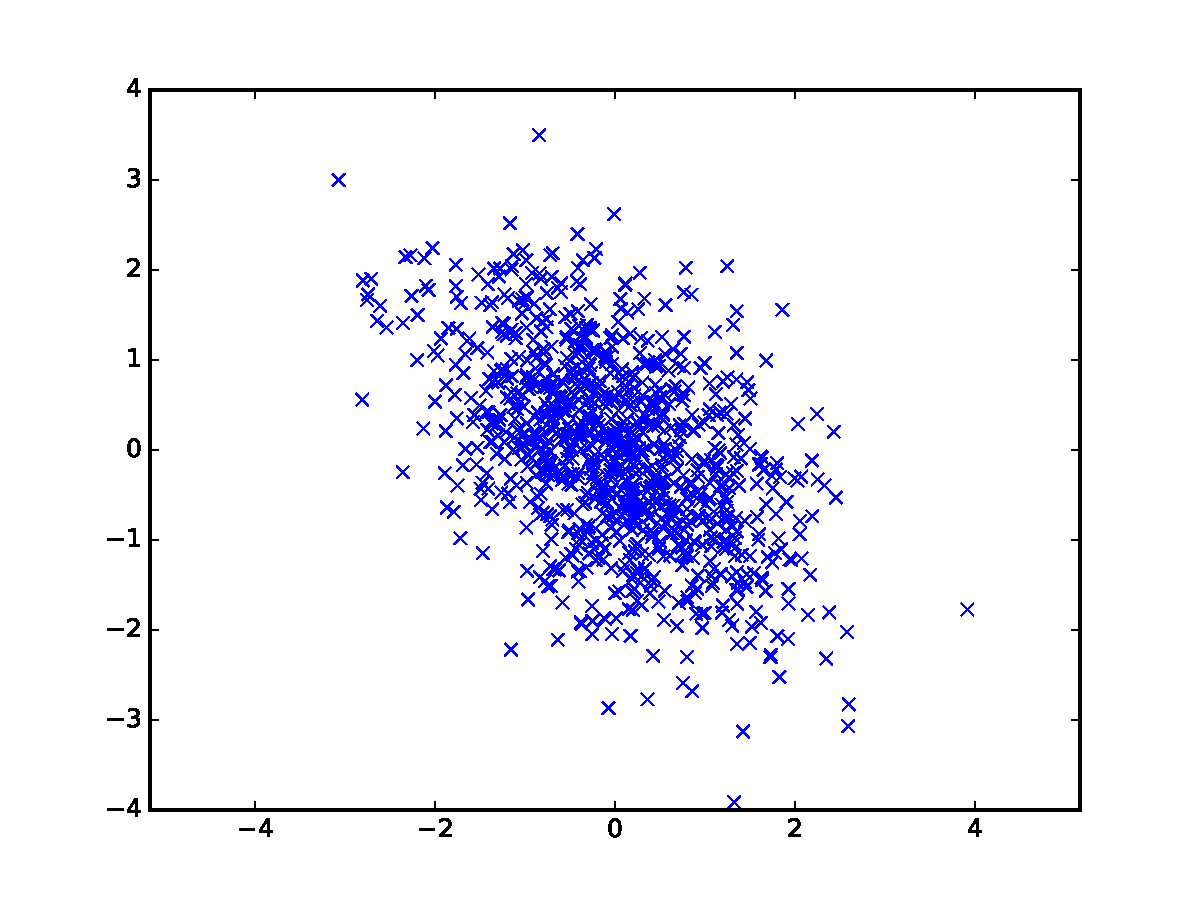
\includegraphics[height=2.5in]{Problem10-e}
                \caption{\(1000\) samples with mean \((0,0)\) and negatively correlated covariance matrix.}
        \end{center}
\end{figure}

\section*{Problem 11}



\section*{Problem 12}

\end{document}